\section{Implementation}\label{sec:impl}

This section introduces our JavaScript
conformance test synthesizer supporting $k$-FS and $k$-FCPS coverage criteria
and explains how it can detect conformance bugs in JavaScript implementations.

%----------------------------------------%
%----------------------------------------%

\subsection{Overall Structure}\label{sec:overall}

\begin{figure}
  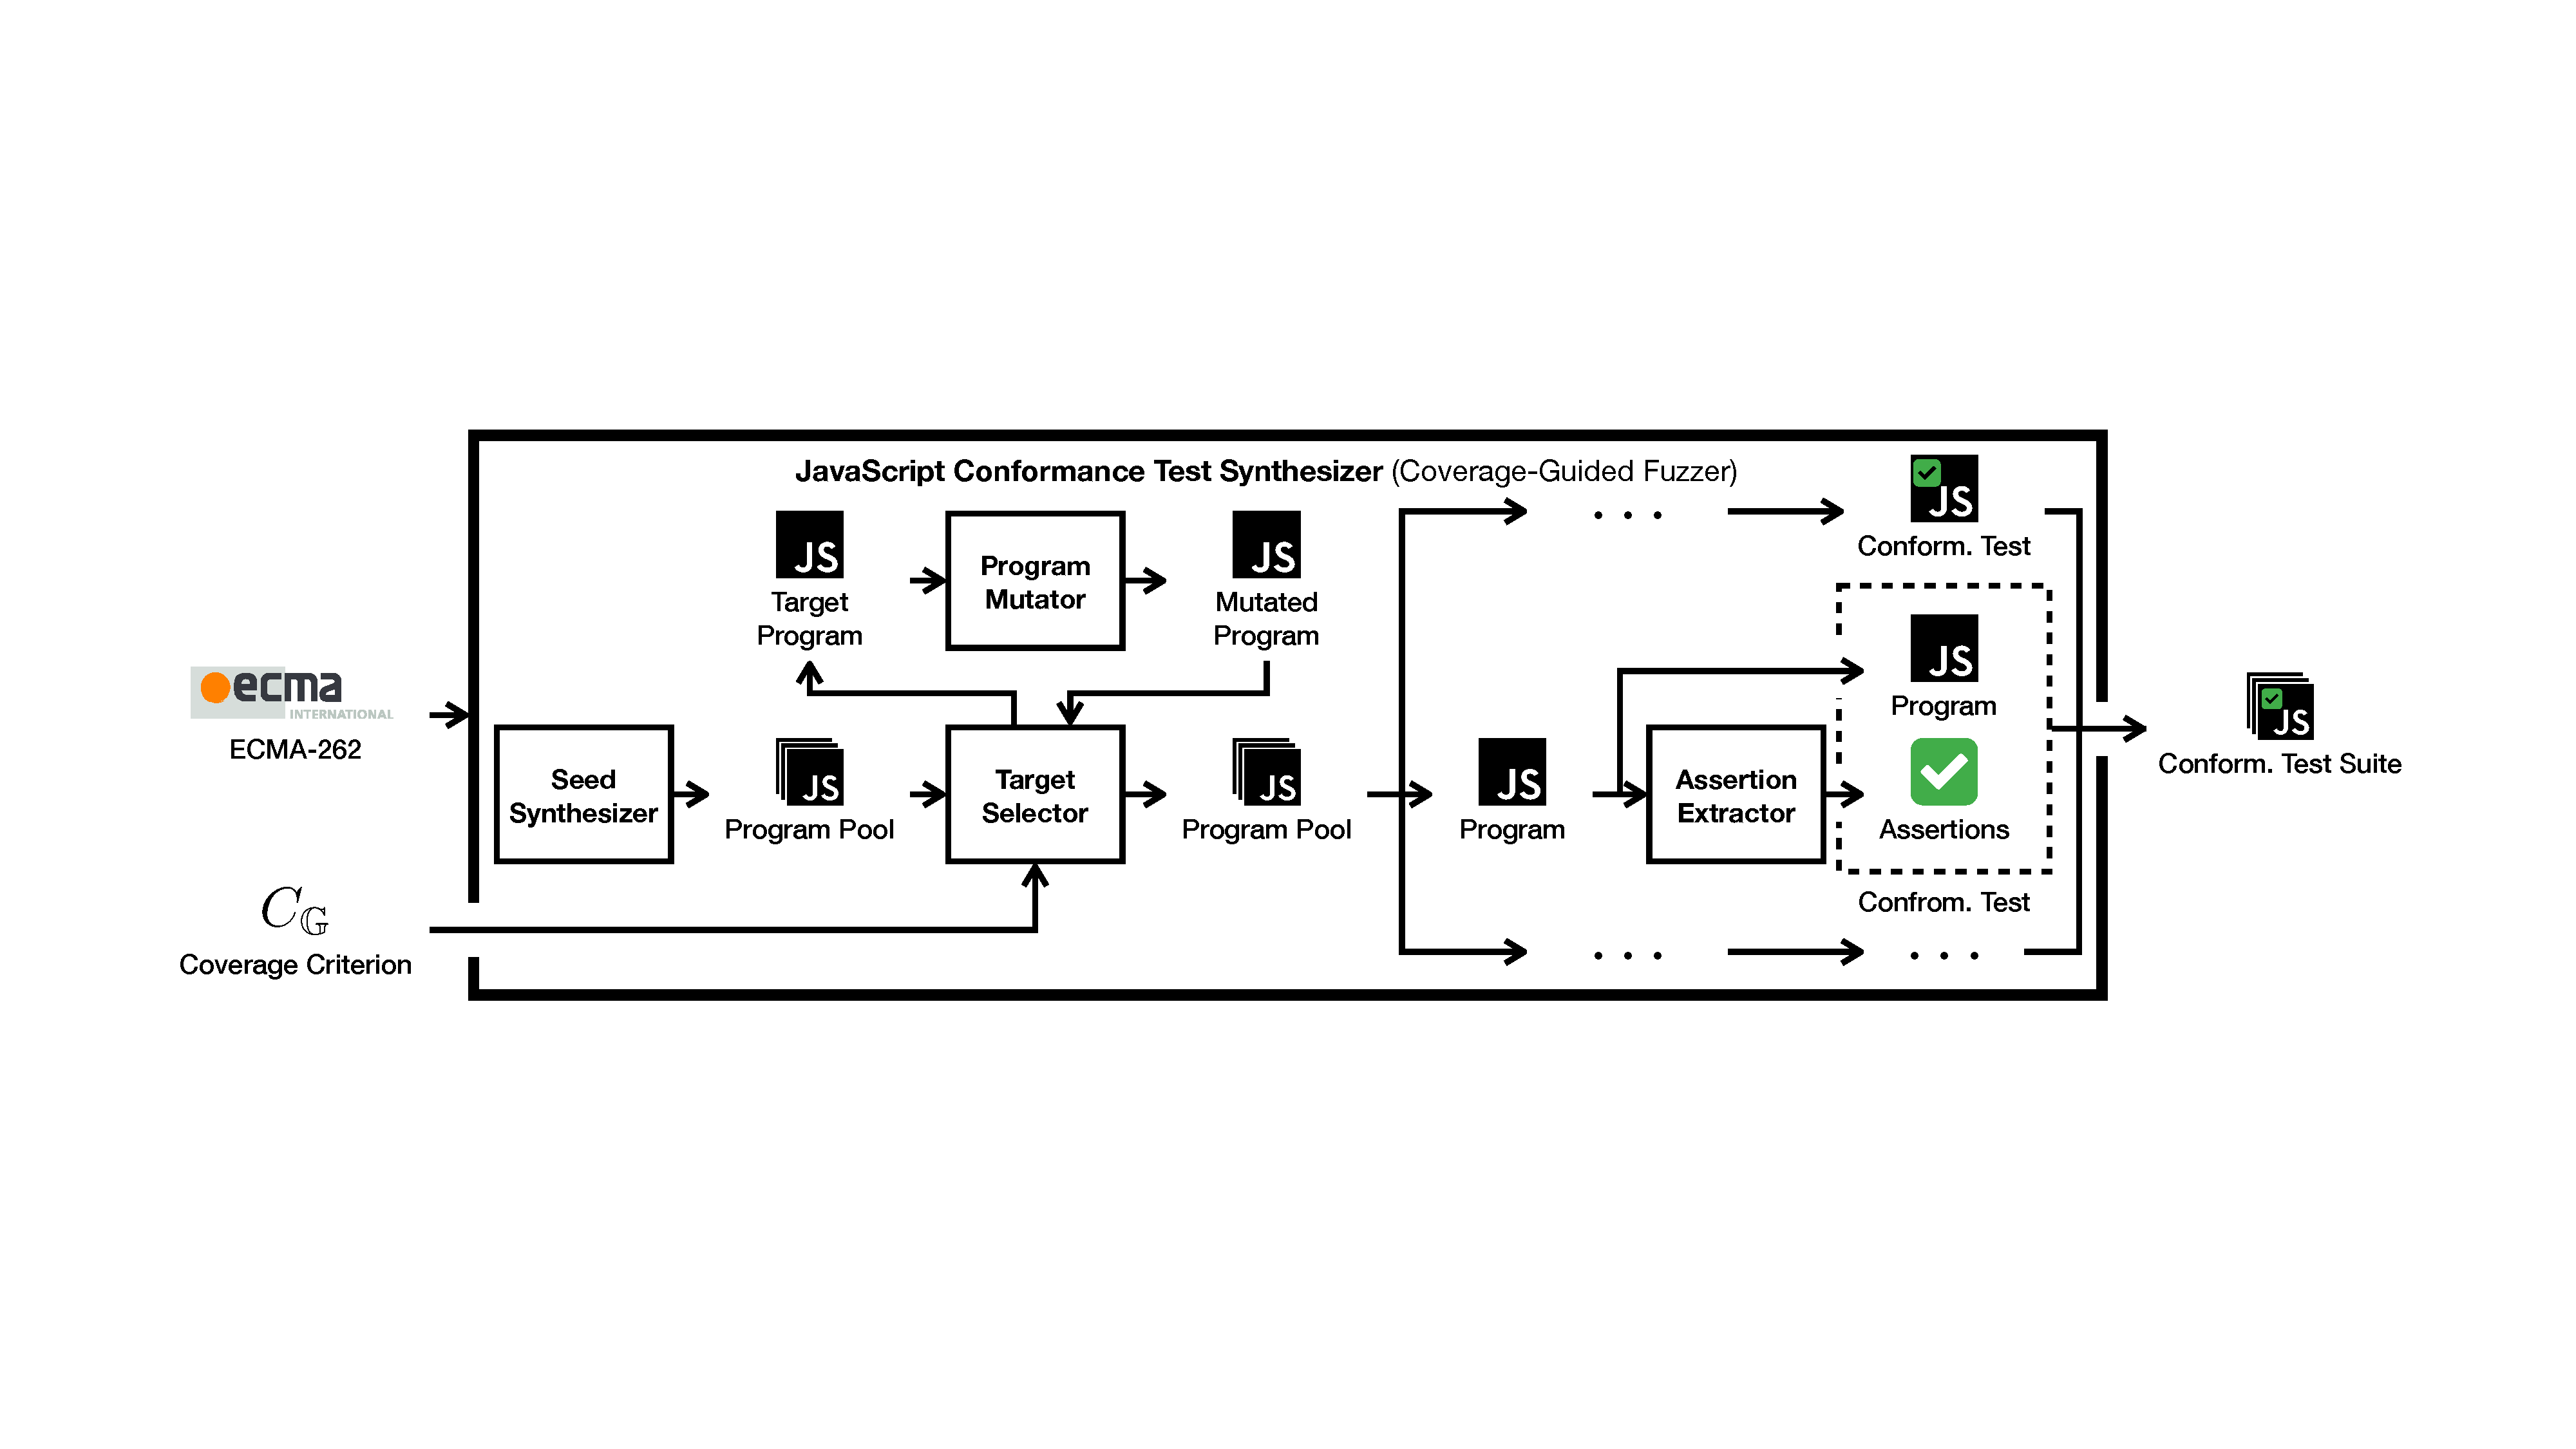
\includegraphics[width=\textwidth]{img/overall}
  \caption{
    Overall structure of a JavaScript conformance test synthesizer using
    coverage-guided fuzzing with the CFG of a mechanized specification
    extracted from the language specification, ECMA-262
  }
  \label{fig:overall}
\end{figure}

Figure~\ref{fig:overall} illustrates the overall structure of $\tool$,
an extension of the state-of-the-art JavaScript conformance synthesizer $\jest$~\cite{jiset}
to support $k$-FS and $k$-FCPS coverage criteria.
$\jest$ uses $\esmeta$\footnote{
  See \url{https://github.com/es-meta/esmeta}
} to automatically extract a mechanized specification from ECMA-262.
$\tool$ takes 1) the extracted mechanized specification
and 2) a coverage criterion $\cov{\graph}$ and performs
coverage-guided fuzzing~\cite{afl} using the CFG of the mechanized specification.
We show the extension in red.


%----------------------------------------%


$\tool$ consists of four modules:
\begin{itemize}
  \item \textsf{\textbf{Seed Synthesizer}}:
    As the first step, \textsf{Seed Synthesizer} automatically synthesizes a set
    of JavaScript programs as the initial \textit{program pool}.
    It uses the JavaScript syntax described in the language specification to
    cover diverse alternatives in syntactic productions.
    $\tool$ uses two existing synthesizers: 1) a non-recursive synthesizer and
    2) a built-in synthesizer.
    %
  \item \textsf{\textbf{Target Selector}}:
    %
    To measure the coverage in the CFG, \textsf{Target Selector} extracts the
    execution path of each program in the pool by interpreting it using the
    abstract algorithms in the specification.
    %
    While the baseline tool supports only a node-or-branch coverage criterion,
    we extend it to support $k$-FS and $k$-FCPS node-or-branch coverage
    criteria as well.
    %
    If a program does not cover new TRs, it removes the program from the pool.
    %
    Then, it selects a program in the pool as a mutation target that potentially
    increases the coverage or stops the iteration when the current status
    satisfies the termination condition.
    %
  \item \textsf{\textbf{Program Mutator}}:
    %
    To increase the coverage in the CFG, \textsf{Program Mutator} repeatedly
    tries to mutate a JavaScript program to a new one using mutation methods.
    %
    $\tool$ uses five mutation methods: 1) random mutation, 2)
    nearest syntax tree mutation, 3) string substitution, 4) object
    substitution, and 5) statement insertion.
    %
  \item \textsf{\textbf{Assertion Extractor}}:
    %
    After the mutation iteration, \textsf{Assertion Extractor} automatically
    extracts seven kinds of assertions from each program in the pool.
    %
    The assertions represent the expected final state of each program according
    to the semantics described in the specification.
    %
    As a result, each pair of a program and the corresponding extracted
    assertions is a \textit{conformance test} for JavaScript.
\end{itemize}

%----------------------------------------%

\begin{figure}
  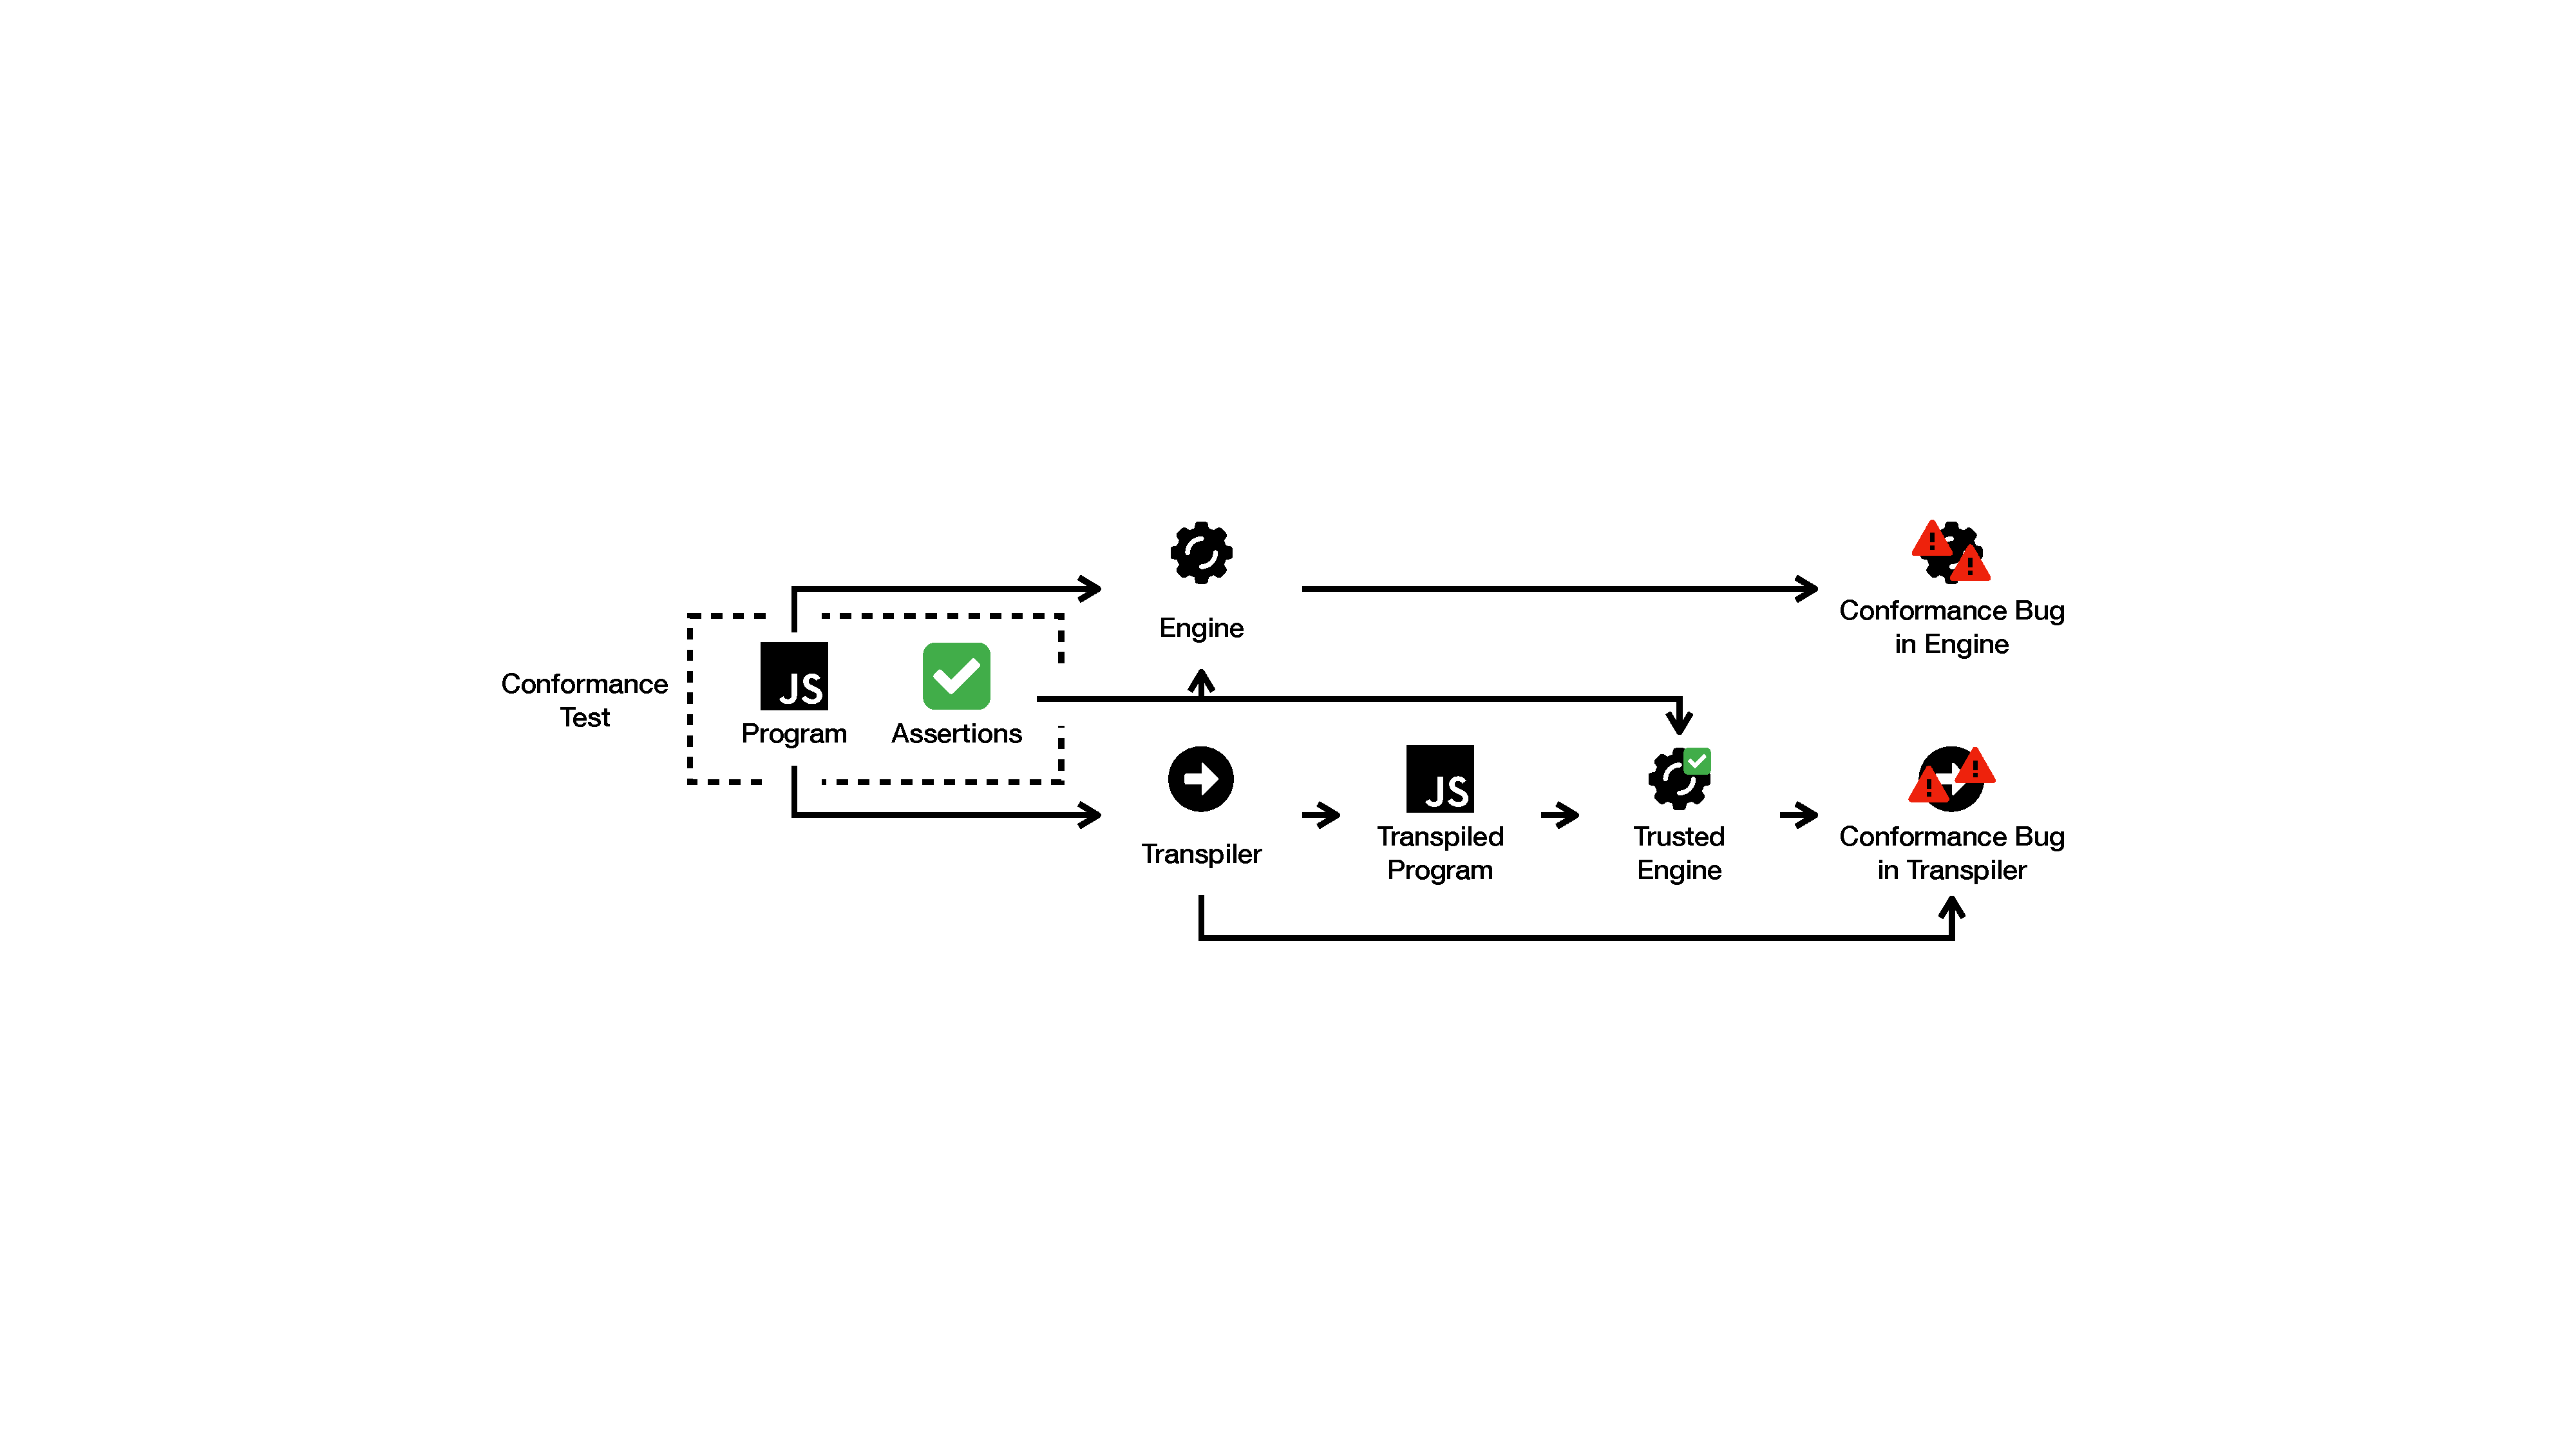
\includegraphics[width=\textwidth]{img/conform-check}
\vspace*{-1.5em}
  \caption{
    Conformance check of JavaScript engines and transpilers with synthesized
    conformance tests
  }
  \label{fig:conform-check}
\end{figure}

%----------------------------------------%
%----------------------------------------%

\subsection{Conformance Check of Engines and Transpilers}
%
A synthesized conformance test consists of a JavaScript program and
corresponding assertions.
Figure~\ref{fig:conform-check} depicts how to use it to check the conformance of
JavaScript engines and transpilers.

To check a JavaScript engine's conformance,
it is enough to run the program in the test and assertions together using the target engine.
If at least one assertion fails, the target engine has a conformance bug related to the test.

To check a JavaScript transpiler's conformance,
we should transpile the program in the test using the target transpiler.
If the transpiler abnormally terminates, it has a conformance bug because
programs in conformance tests are valid.
Otherwise, we should run the transpiled program and assertions together
using a trusted engine.
Like the engine conformance checking, the target transpiler has a conformance bug
related to the test if at least one assertion fails.
